\documentclass{report}
\usepackage[utf8]{inputenc}
\usepackage[english]{babel}
\usepackage{url}
\usepackage[hidelinks]{hyperref}
\usepackage{graphicx}
\usepackage{float}
\usepackage{booktabs}
\title{}
\date{\today}
\author{Johanna Sörbom}

\newcommand{\case}[1]{\subsubsection*{#1}}
\newcommand{\ac}{AC-system}
\newcommand{\cmp}[2]{\ensuremath{#1+#2i}}
\newcommand{\mypart}[2]{\section*{Part #1 - \textit{#2}}}
\newcommand{\mysubpart}[1]{\subsection*{#1}}
\begin{document}
\maketitle
\chapter*{Introduction}
\chapter*{Method}
\chapter*{Background}
\chapter*{Result and calculations}
\mypart{A}{How}
\mysubpart{Impedance of power lines}
The impedence of the power line is given by the equation 

\begin{equation}\label{eq_impd}
Z =  L \cdot Z_{km}
\end{equation} where $L$ is the length of the power line in kilometers and $Z_{km}$ is the impedience per kilometer in Ohms.

\case{Ställverket to Brytpunkten}
For the case of Ställverket to Brytpunkten, we have $L=10km$ and $Z_{km}=\cmp{0.2}{0.4}$.  We get,

\begin{eqnarray}
Z&=&  L \cdot Z_{km} \\
&=&10 (\cmp{0.2}{0.4}) \\
&=& \cmp{2}{4} \label{res1}
\end{eqnarray} by substituing into equation \ref{eq_impd}. Interpreting the real part of the result obtained in equation \ref{res1} as resistance and the complex part as reactance, we have $R=2\Omega$ and $X=4\Omega$ respectively.

\case {Brytpunkten to Framtiden}
For the case of Brytpunkten to Framtiden, we have $L=15km$ and $Z_{km}=\cmp{0.2}{0.4}$.  We get,

\begin{eqnarray}
Z&=&  L \cdot Z_{km} \\
&=&15 (\cmp{0.2}{0.4}) \\
&=& \cmp{3}{6} \label{res2}
\end{eqnarray} by substituing into equation \ref{eq_impd}. Interpreting the real part of the result obtained in equation \ref{res2} as resistance and the complex part as reactance, we have $R=3\Omega$ and $X=6\Omega$ respectively.

\case {Brytpunkten to Solsidan}
For the case of Brytpunkten to Solsidan, we have $L=21.21km$ and $Z_{km}=\cmp{0.2}{0.4}$.  We get,

\begin{eqnarray}
Z&=&  L \cdot Z_{km} \\
&=&21.21 (\cmp{0.2}{0.4}) \\
&=& \cmp{4.24}{8.49} \label{res3}
\end{eqnarray} by substituing into equation \ref{eq_impd}. Interpreting the real part of the result obtained in equation \ref{res3} as resistance and the complex part as reactance, we have $R=3\Omega$ and $X=6\Omega$ respectively.

\case {Framtiden to Solsidan}
For the case of Framtiden to Solsidan, we have $L=15km$ and $Z_{km}=\cmp{0.3}{0.1}$.  We get,

\begin{eqnarray}
Z&=&  L \cdot Z_{km} \\
&=&15 (\cmp{0.3}{0.1}) \\
&=& \cmp{4.5}{1.5} \label{res4}
\end{eqnarray} by substituing into equation \ref{eq_impd}. Interpreting the real part of the result obtained in equation \ref{res4} as resistance and the complex part as reactance, we have $R=4.5\Omega$ and $X=1.5\Omega$ respectively.

\case {Vindeby to Solsidan}
For the case of Vindeby to Solsidan, we have $L=15km$ and $Z_{km}=\cmp{0.3}{0.1}$.  We get,

\begin{eqnarray}
Z&=&  L \cdot Z_{km} \\
&=&15 (\cmp{0.2}{0.4}) \\
&=& \cmp{3}{6} \label{res5}
\end{eqnarray} by substituing into equation \ref{eq_impd}. Interpreting the real part of the result obtained in equation \ref{res5} as resistance and the complex part as reactance, we have $R=3\Omega$ and $X=6\Omega$ respectively.

\mysubpart{Reactive power}
Complex power is defined as, \begin{equation}
S = \sqrt{P^2 - Q^2} \label{s}
\end{equation}
where $P$ is the active power and $Q$ is the reactive power. For balanced load in an \ac we have, 
\begin{equation}
P = S \cdot \cos\theta
\end{equation}
where $\theta$ is the phase offset between voltage and current. 

\case{Brytpunkten}
For the case of Brytpunkten where $\cos\theta = 0.9$ and $P = 35 MW$ we get,
 
\begin{eqnarray}
Q&=&   = \sqrt{S^2 - P^2}\\
&=& \sqrt{38.89^2 - 35^2} \\
&=& 16.95 MW \label{res}
\end{eqnarray} 
by substituting into equation \ref{s}.

\case{Framtiden}
For the case of Framtiden where $\cos\theta = 0.9$ and $P = 10 MW$ we get,
 
\begin{eqnarray}
Q&=&   = \sqrt{S^2 - P^2}\\
&=& \sqrt{11.11^2 - 10^2} \\
&=& 4.84 MW \label{res}
\end{eqnarray} 
by substituting into equation \ref{s}.

\case{Solsidan}
For the case of Solsidan where $\cos\theta = 0.9$ and $P = 5 MW$ we get,
 
\begin{eqnarray}
Q&=&  \sqrt{S^2 - P^2}\\
&=& \sqrt{5.56^2 - 5^2} \\
&=& 2.43 MW \label{res}
\end{eqnarray} by substituting into equation \ref{s}.

\mysubpart{Voltage in power lines}
By using Excell to calculate the voltage in the power lines using data from above we get two cases.

\case{Not using wind power or solar power}
Not using wind power or solar power results in the following voltage in the power lines. 

\begin{table}[H] 
\begin{tabular}{ll}
\toprule
Location & Voltage (kV) \\
\midrule
Brytpunkten & 67.00\\
Framtiden  &  66.18\\
Solsidan & 66.26\\
\bottomrule
\end{tabular} 
\end{table} 

As seen in figure \ref{fig_utan_vindeby}
\begin{figure}[h]
\label{fig_utan_vindeby}
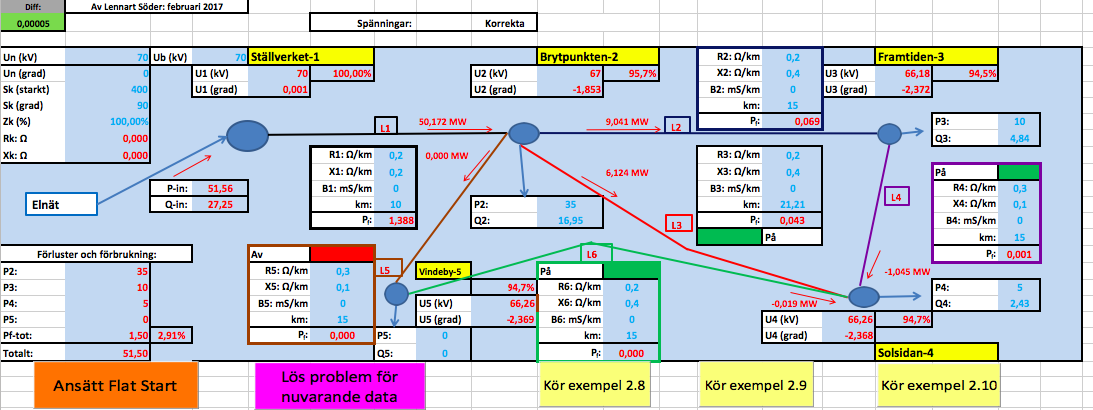
\includegraphics[width=\linewidth]{utan_vindeby.png}
\caption{Voltage when using wind power from Vindeby.} 
\end{figure}

\case{Using wind power but not solar power}
Using wind power but not solar power results in the following voltage in the power lines, 

\begin{table}[H] 
\begin{tabular}{ll}
\toprule
Location & Voltage (kV) \\
\midrule
Brytpunkten & 65.72 \\
Framtiden  &  64.15\\
Solsidan & 63.5\\
\bottomrule
\end{tabular} 
\end{table}

As seen in figure \ref{fig_med_vindeby}
\begin{figure}[h]
\label{fig_med_vindeby}
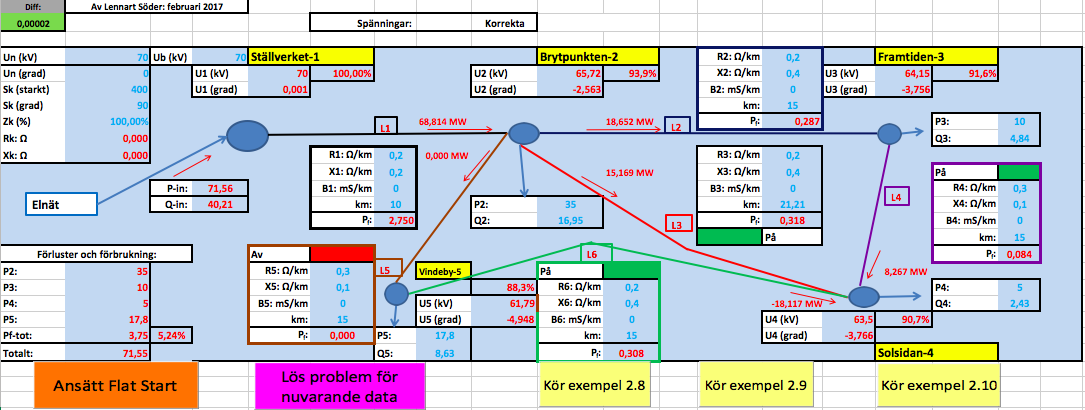
\includegraphics[width=\linewidth]{med_vindeby.png}
\caption{Voltage when not using wind power.} 
\end{figure}





\end{document}
